\chapter{Introduction}\label{ch:introduction}
\section{Reversible adhesion: current challenges}\label{sec:current_challenges}
\section{Existing solutions}\label{sec:existing solutions}
\section{Bio inspired approach to reversible adhesion}\label{sec:bio_inspired_approach}
\subsection{Tree frog adhesive mechanisms}\label{sec:tree_frog_adhesion}
\subsubsection{Morphology}
\qquad Tree frogs use the so-called mechanism of wet adhesion to adhere to surfaces in their living environment. Animals using wet adhesion use fluids to increase their adhesional performance and tree frogs do so by secreting watery mucus. The exact functionality of the mucus secreted by tree frogs is not yet clear. Studies show that both viscous forces and surface tension are likely to contribute to the adhesional performance of the tree frog \cite{hanna1991adhesion}. Adhesional performance is furthermore dependent on the compliance of the adhesional pads. Adhesional pad compliance is relevant for all animal that make use of reversible adhesion. The compliance of the adhesional pads is dependent on morphological properties of the pads used by animals to adhere to a surface. The morphological properties of the digital digits of the different species of tree frogs described in literature are very similar. In fact, it is usually not possible to identify the family from the appearance of the toe pads \cite{barnes2011elastic}. The morphological properties described below are from observations on the \textit{Litoria Caerulea White} by Scholz et al. and by Barnes et al. \cite{scholz2009ultrastructure,barnes2011elastic} and on the \textit{Osteopilus Septentrionalis} by Hanna et al. \cite{hanna1991adhesion}.\\

\qquad A study by Langowski et al.\cite{langowski2018force} reveals the morphological properties of the \textit{Hyla Cinerea}. This study does not only analyze the epidermal properties but also gives insight in the dermal structure of the tree frog digits. The morphological properties of the rock  frog \textit{Staurois Parvus} described by Drotlef et al. \cite{drotlef2015morphological} are slightly different from the properties of the \textit{Hyla Cinerea}.\\ 

% Epidermal structure, over de zeskantige cellen
\qquad The specialised adhesive pad epithelium of the \textit{Hyla Cinerea} is 10- to 15 \textmu m thick and delineated from the normal skin by distinct grooves. The epidermis consists of four to six layers of columnar epithelial cells. The outermost layer is non-living and consists out a polygonal epithelial cells. Most of these are hexagonal but pentagonal, heptagonal an octagonal formed epithelial cells are also observed. The structure of the second cell layer is very similar to the structure of the outer cell layer. This layer will become the outer layer when the first layer has worn of. The epithelial cells contain keratin fibrils with are oriented at an angle to the surface. For both tree frogs and rock frogs the fibrillar structures in the epithelial cells are distally pointed.\\ 

\qquad The amount of angling varies between species: for some species the fibrillar structure is almost normal tot the surface while for other species like the \textit{Hyla Cinerea} as described by Langowski et al.\cite{langowski2018force}, the fibrillar structures are more angled as is visible in Figure \ref{fig:epidermal_structures_all}. The nanopillars on top of the epithelial cells are formed from the end of these keratin filaments and (partly) fill these structures. The presence of the keratin filaments increases the stiffness of and the wear resistance of the epithelial cells and the nanopillars on top of these and the angling of the keratin filaments gives the adhesive pad directional dependent properties.\\ 

% over de afmetingen van de epithelial cells en channels ertussen
\qquad The epithelial cells have a diameter of 13 \textmu m. A network of channels exists between the epithelial cells. This channel network follows the hexagonal pattern of the epithelial cells for the tree frogs. The adhesive pads of the rock frogs however has more stratified channels which form a shorter route to the channel running around the toe pads. The channels between the epithelial cells for both tree frogs and rock frogs have a width of about 1-2 \textmu m and are about 10 \textmu m in depth. The channel surrounding the toe pad not only functions in drainage of excess water from the pad but is also ideally placed to channel fluid around rather than under the pad.

\begin{figure}[h!]
     \begin{subfigure}{0.45\textwidth}
         \centering
         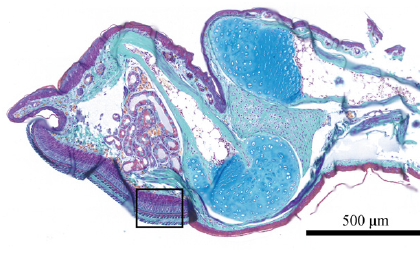
\includegraphics[width=\linewidth, height=5.5cm, angle=0]{images/epidermal structure/epidermis_langowski_1.png}
         \caption{}
         \label{fig:toe_pad_section}
     \end{subfigure}
     \hfill
     \begin{subfigure}{0.45\textwidth}
         \centering
         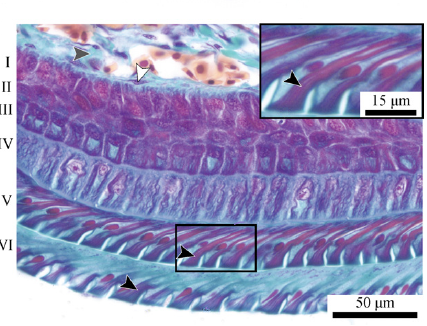
\includegraphics[width=\linewidth, height=5.5cm, angle=0]{images/epidermal structure/epidermis_langowski_2.png}
         \caption{}
         \label{fig:epidermis_different_levels}
     \end{subfigure}
     \hfill
    \caption{Pictures from the paper by Langowski et al. \cite{langowski2018force} which show the epidermal structure to the level of the epithelial cells. (a) A mid-sagittal section of a digital pad of the Hyla Cinerea. (b) A magnified view of the ventral epidermis. The cellular layers are visible and numbered with the numbers \rom{1}-\rom{6}. The fibrillar structure has a reddish colour and is better visible in the magnified view in the top right of the image. The black arrows point to the fibrillar structure in the epithelial cells, the white arrows to the reticular cells and the grey arrows point to the reticular connective tissue.}
    \label{fig:epidermal_structures_all}
\end{figure}


% over de nanopillars 
\qquad The surfaces of the epithelial cells are covered with closely packed columnar nanopillars. The dimensions of these pillars vary between species and measures 200 nm to 350 nm in diameter for the frog species \textit{Osteopilus Septentrionalis} and \textit{Staurois Parvus}. The height of the nanopillars for these frogs is 300 - 500 nm which gives the pillars an aspect ratio between 1 and 2. The nanopillars of the \textit{Litoria Caerulea} are smaller with a diameter and height of approximately 22 nm.\\ 

\qquad The nanopillars as visible in Figure \ref{fig:nanopillars} do contribute to the frictional and adhesive properties of the adhesive pads. The most probable mechanism for this performance enhancement is that the nanopillars allow for close conformation to surface irregularities. Just as the epithelial cells, but at a much smaller length scale. This close conformation activates Van der Waals forces and increases capillary forces through thinning of the fluid layer between adhesive pad and substrate. The close surface conformation is mainly caused by by the presence of the grooves surrounding each nanopillar and by the compliance of the pillars caused by the low stiffness of the pillars and by their aspect ration which allows them to bend easily. The nanopillars mainly effect the frictional forces which come close to dry frictional forces due to the close contact made between the adhesive pad and surface. Their role in capillary forces is expected to be much less since such forces are generated by the air-water interface around the edge of the pad \cite{ernst1973digital}.\\

\qquad The nanopillars each have a slight depression or ‘dimple’ on top of each pillar. This dimple has a depth of approximately 6-8 nm and the edges of these dimples are interrupted with one or two channels connecting the dimple with the surrounding space between the nanopillars. Between the nanopillars are channels. These channels form a part of the channel network on the adhesive pads which drains excess water from the pads and acts as a reserve to make capillary adhesion possible on dry surfaces. The channels connecting the dimples with the channels around the nanopillars extend this channel network.\\ 

\begin{figure}[h!] 
\begin{subfigure}{0.48\textwidth}
    \centering
    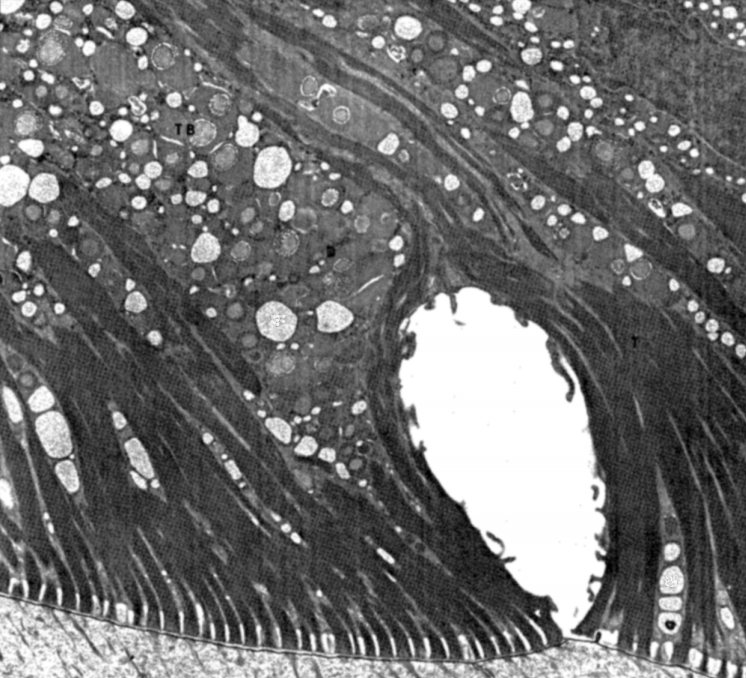
\includegraphics[width=\linewidth, height=6cm, angle=0]{images/epidermal structure/epithelial_cells_and_nanopillars_ernst.PNG}
    \caption{}
    \label{}
\end{subfigure}
\hfill
\begin{subfigure}{0.48\textwidth}
    \centering
    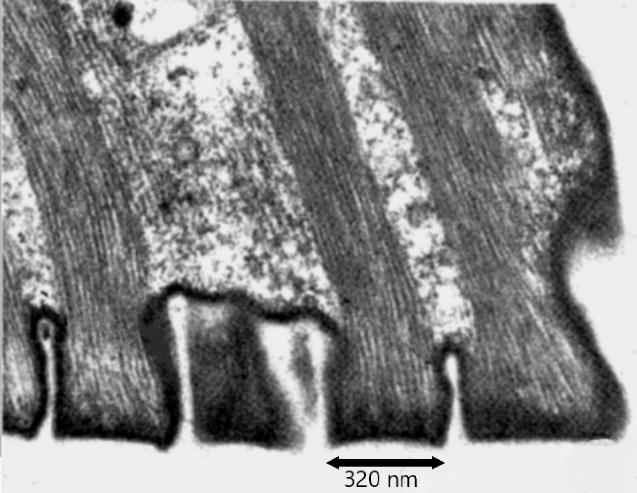
\includegraphics[width=\linewidth, height=6cm, angle=0]{images/epidermal structure/nanopillars_ernst.PNG}
    \caption{}
    \label{}
\end{subfigure}
 \caption{Pictures from the paper by Ernst et al. which show the structures of the adhesive pads of the Hyla cinerea \cite{ernst1973digital}. (a) Epithelial cells on which multiple nanopillars are visible. The dark lines visible are the keratin fibres which originate in the epithelial cells and run up to the surfaces of the nanopillars. (b) Close-up of the nanopillars with a more detailed view on the keratin fibres. The width of one nanopillar as depicted above is an estimation based on the data provided by Ernst et al.}
 \label{fig:nanopillars}
\end{figure}

% over de ventral collogen layer
\qquad The epidermal layer is supported by the dermal structure of the toe digit. In Figure \ref{fig:epidermis_different_levels} are the reticular cells visible. The cells in this layer connect the epidermal structure with the higher level dermal structure, the dermal stratum spongiosum. The amount of keratin fibres reduces with the depth of the epidermis. This confirms the stiffness measurements described above.\\ 

\qquad Scholz et al. describe a decrease in the density of the cytoskeletal elements in the epidermal structure. They describe that the diameters of the pores in the epithelial cell structure are smaller towards the outer surface of the cell. In the deeper cell layers they describe a lose lattice of fibrillar material. This also explains why the outer epidermal structure has a higher stiffness than the underlying material. From the literature available it can be concluded tree frog adhesive pas have a thin but slightly harder ‘skin’, with a Young’s modulus equivalent to silicon rubber, covering a soft gel-like structure.\\ 

\qquad This gel-like structure, the dermal stratum spongoisum has a dense network of capillaries. This capillary network is similar to the blood sinuses that occur beneath the hairy adhesive pads of gecko's and are thought to act as a hydrostatic skeleton maintaining pressure on the scansors that hold the adhesive setae. When the digit is brought in contact with a surface, the phalanx in the digit presses down on the structure between the phalanx and the epidermis. This increases the pressure in the dermal structure above the epidermis and presses the pad on the substrate. It is possible that the tree frog uses its capillary network in the stratum spongiosum in a similar way.\\ 

\begin{figure}[!ht]
    \centering
    \raisebox{-0.5\height}{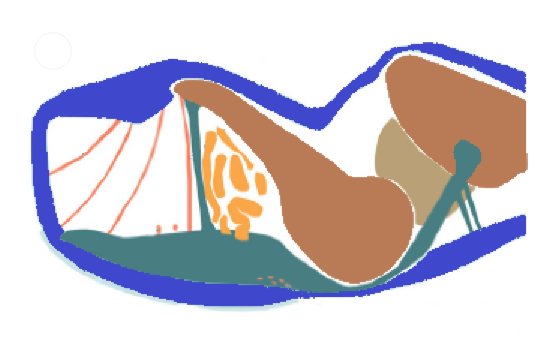
\includegraphics[width=0.45\linewidth, height=5.5cm, angle=0]{images/epidermal structure/schematic_view_voorlopig.PNG}}
    \hspace*{.2in}
    \begin{tabular}{p{0.3cm} p{4cm}}
    \mycbox{blueviolet} & Apical dermis/Basal epidermis\\ 
    \mycbox{lightblue} & Adhesive epidermis\\
    \mycbox{collagen_color} & Collagen material\\ 
    \mycbox{glands_color} & Mucus glands\\
    \mycbox{phalanx_color} & Distal and middle phalanx\\ 
    \mycbox{intercalary_color} & Intercalary element\\
    \mycbox{muscle_color} & Muscle fibers\\
    \end{tabular}
    \captionlistentry[table]{A table beside a figure}
    %\captionsetup{labelformat=andtable}
    \caption{Schematic representation of the dermal structure. This figure is derived from the paper form Langowski et al.\cite{langowski2018force}.}
    \label{fig:dermal_structure}
\end{figure}


\qquad The collagen layer is well described in the work of Langowski et al. This layer fills the space between the epidermis, the gland space and runs below the base of the distal phalanx. Proximal to this base, it converges and connects to the side arms of the collateral ligaments. The collagen ridges gradually flatten and and vanish towards the distal end of the pad. The collagen layer has a fibrous structure and the fibres are oriented along the distal-proximal axis. The collagen layer below the gland space is separated in longitudinal ridges. Mucus ducts and blood vessels occupy the space in the troughs between the ridges. The ridges are not visible in the proximal part of the collagen layer.\\

\qquad The ridges in the collagen layer compensate for the loss in tensile strength caused by the the mucus ducts which perforate the collagen layer and with that, weaken its structural integrity. This is also confirmed in the paper by Langowski et al. in which is shown that the ridges are oriented along the trajectories of the maximum stresses along the ventral surface of the adhesive pad. It is also quite probable that the collagen layer has a lower stiffness in the transverse direction than in the longitudinal direction. The stresses for which the collagen layer is optimally designed occur when the ventral surface is loaded by proximal shear along the ventral pad surface.\\ 
    
\qquad The dermal pad structure is divided in two parts by a septum that runs from the distal tip of the phalanx towards the ventral epidermis. In the distal compartment the dermal stratum spongiosum can be found which has a very soft structure due to lymph filled spaces that are present in this compartment. Furthermore, there are two types of muscle fibres present in the space distal to the collagenous septum: in Figure \ref{fig:dermal_structure} a group of muscle fibres is visible which is oriented in ventral-dorsal direction. Another group of cross-lateral muscle fibres is also visible in Figure \ref{fig:dermal_structure}. There are two distinct thick muscle fibres that run from the tip of the distal phalanx to the ventral collagen layer. Although most muscle fibers are located in the distal lymph space, there is also one group of cross-lateral muscle fibers proximal to the collagenous septum. These muscle fibres are embedded in the collagen layer discussed above.\\ 
\qquad The dermal structure proximal to the collagenous septum contains numerous mucus glands. The glands in this gland space are all connected to the ventral pad surface via mucus ducts that traverse the dermal structure. These ducts lie in the troughs between the ridges of the collagen layer discussed above.\\

\subsubsection{Behavioural adaptions}\label{sec:intro_spreading}
\qquad A study performed by Endlein et al. \cite{endlein2013sticking} shows that tree frogs actively change their position when higher adhesional forces are required. The tree frogs change their position to a sprawled position by extending their legs laterally. This reduces the contact angle between pads and substrate and increases the lateral forces between at the contact interface. This spreading is visible in Figure \ref{fig:tree_frog_limb_spreading}. 

\begin{figure}[h!] 
\begin{subfigure}{0.32\textwidth}
    \centering
    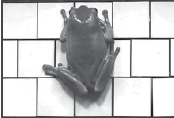
\includegraphics[width=\linewidth, height=4cm, angle=0]{images/limb spreading/Tree_frog_spread_rest_endlein2013sticking.png}
    \caption{}
    \label{fig:limb_spreading_rest}
\end{subfigure}
\hfill
\begin{subfigure}{0.32\textwidth}
    \centering
    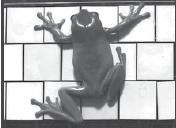
\includegraphics[width=\linewidth, height=4cm, angle=0]{images/limb spreading/Tree_frog_first_spread_endlein2013sticking.png}
    \caption{}
    \label{fig:limb_spreading_first_spread}
\end{subfigure}
\begin{subfigure}{0.32\textwidth}
    \centering
    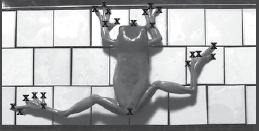
\includegraphics[width=\linewidth, height=4cm, angle=0]{images/limb spreading/Tree_frog_second_spread_endlein2013sticking.png}
    \caption{}
    \label{fig:limb_spreading_second_spread}
\end{subfigure}
  \caption{Stages in the limb spreading of the tree frog on inclined surfaces \cite{endlein2013sticking}. (a) The initial position of the resting frog. (b) The first spread of the frog. (c) The second spread of the frog.}
  \label{fig:tree_frog_limb_spreading}
\end{figure}

\qquad There are two stages visible in this limb spreading: the frog first spreads its limbs when adhesional performance in the resting position is insufficient (Figure \ref{fig:limb_spreading_first_spread}). The frog spreads its limbs even further when the adhesional performance in the first spread is insufficient (Figure \ref{fig:limb_spreading_second_spread}). The impact of this spreading behaviour is further described in Section \ref{sec:behavioral analysis}. 

\qquad The magnitude of the forces involved in the proximal pulling are visible in Figure \ref{fig:mag_pulling}. This figure shows that the magnitude of the proximal pulling force has a maximum value of approximately one-fifth of the body weight. The large variation visible in the results of Endlein et al. however, does not allow for an accurate estimation of the pulling force magnitude. 

\begin{figure}
    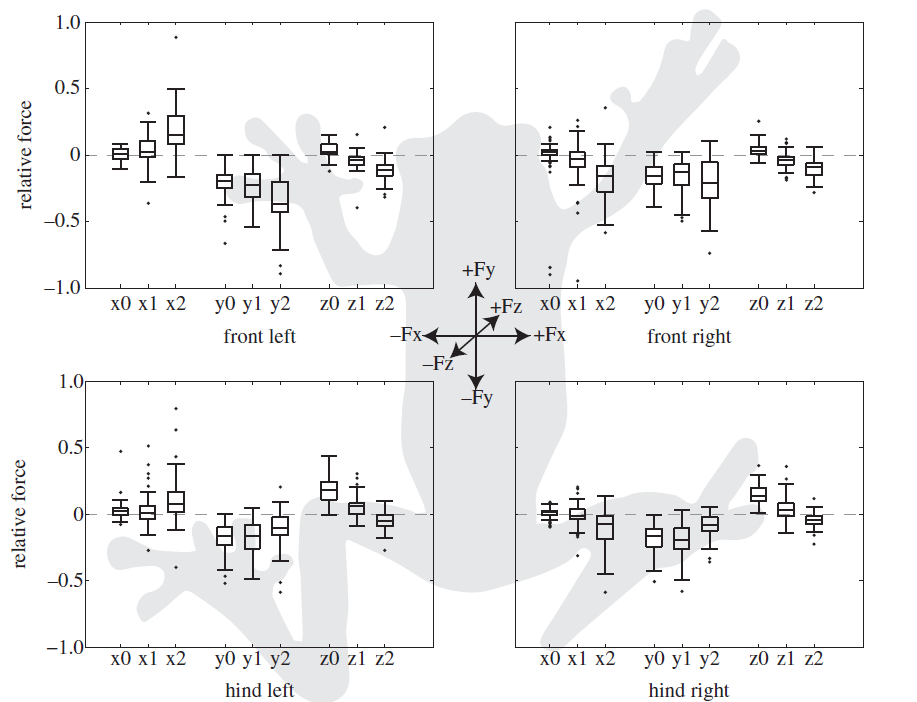
\includegraphics[width=0.65\linewidth, height=7cm, angle=0]{images/limb spreading/work_endlein.PNG}
    \caption{Relative force as force per body weight generated at the interface of the individual limbs. The resting position, first and second spread is indicated by the indexes 0, 1 and 2 respectively.}
    \label{fig:mag_pulling}
\end{figure}







\subsubsection{Bio material properties}\label{sec:bio_material_properties}
The epidermal structure of the tree frog is composed of different bio-materials. The exact composition this structure is known to be dependent on the age of the animal \cite{barnes2011elastic} and it furthermore likely to be dependent on species and living environment as it is for other animals \cite{peng2016microstructure}. The adhesional performance of the animal is dependent on the mechanical properties of the adhesive pads. Actual measurements of these properties are described in studies by Barnes et al. and in work from Scholz et al. \cite{barnes2005mechanical,scholz2009ultrastructure,barnes2011elastic,barnes2013comparative,kappl2016nanoscale}. The results from the stiffness measurements are visible in Table \ref{tab:experiments_literature}. The content of this table matches the content published by Langowski et al. \cite{langowski2018tree}. The Young's modulus of the adhesive pads is found to be inversely proportional to the indentation depth. This behaviour makes the toe epidermis self-adaptive to an applied load. The pads show pure elastic deformation indented more than $200 \mu m$ \cite{barnes2011elastic}. Furthermore, the toe pad epithelium is found to be stiffer than the dermal material directly under the epithelium. 


\begin{table}[h!]
\hspace*{-1cm}\begin{tabular}{p{2cm}|p{2cm}|p{1.5cm}|p{1.5cm}|p{1.5cm}|p{1.5cm}|p{1.5cm}|p{1.5cm}|p{2cm}}
Species & Setup & Diameter indentor [$\mu m$] & Indentation depth [$\mu m$]  & Frequency [Hz] & Indentation velocity [$\mu m$] & Stiffness mean value [kPa] & Work of adhesion [$J/m^2$] & Source\\ 
\hline
Litoria Caerulea & Whole frog with restricted limbs, temporally anesthetized & & 1.6 & 1-2 & 3.2-6.4 & 5.7e3 & & Scholz 2009\\
\hline
Litoria caerulea & & & 50 - 350 & & & 12 & & Barnes 2005\\
\hline
Litoria Caerulea & Whole frog with restricted limbs, temporally anesthetized & 1500 & 350 & 1/35, 5 s relaxation time & 23 & 4.45 & 0.08 & Barnes 2011 \\
\hline
Litoria Caerulea & Toes removed from frogs & 0.04 & 0.2 & 0.5 & & 33.5& & Barnes 2013\\
\hline
Rhacophorus Prominanus & Toes removed from frogs & 0.04 & 0.2 & 0.5 & & 28.7 &  & Barnes 2013  
\end{tabular}\hspace*{-1cm}
\caption{Setup and results from indentation experiments described in literature}
\label{tab:experiments_literature}
\end{table}


\qquad In Table \ref{tab:experiments_literature} is visible that the stiffness values found for the experiments described by Scholz are much higher than the values found in the studies of Barnes et al. In the paper published by Barnes in 2011, the author ascribes the the higher measured stiffness in the study by Scholz et al. to the the difference in indentation depth between the experiment carried out by Scholz and the experiment carried out by Barnes in 2011. The experiments by Barnes et al. from 2013 however, use a similar technique and indentation depth as used by Scholz et al. in 2009 and still report much lower values for the stiffness than reported by Scholz et al. Possible other explanations between this difference in measured stiffness are:
 \begin{itemize}
     \item The indentation frequency used in the experiments of Scholz is higher. This can allow viscoelastic effects to play a role. The stiffness of most viscoelastic materials increases with an increase in loading frequency. 
     \item The experiment by Barnes et al. from 2013 involves tree frog toes that are separated from the animal while the experiment by Scholz et al. involves living tree frogs. Measurements on living tissue are more sensitivity to animal induced distortions such as the animals heart beat. 
     \item For the study by Barnes et al., the cut-off limbs were placed in a Ringer's solution. This solution can soften the epithelial tissue, especially the outer layer of the cellular layers. This effect can play a significant role since the indentation depth is relative small in the experiment by Barnes et al. from 2013. 
     \item It is known that the stiffness of epithelial material increases with the age of the tree frog \cite{barnes2011elastic}. A difference in age between the frogs used by Barnes and Scholz could play a role in the difference in measured stiffness between these two studies. 
     \item The mathematical models to calculate the stiffness from the indentation data differs between the studies under consideration. Barnes describes a modified version of the Hertz contact model while Scholz has uses a force-indentation model form Oliver and Parr. Both models can be used to calculate stiffness values but it is possible that these models produce different results for similar input data. 
 \end{itemize}
 
 \qquad As a consequence of the relatively large difference between the reported values of the stiffness of the adhesive pads, the stiffness of these pads needs to based on a choice of one of the values reported in literature while neglecting the other. The stiffness values reported by Barnes et al. are considered the most reliable because:
 \begin{itemize}
     \item The stiffness values reported in the three individual papers by Barnes et al. are all in the same range while each individual paper reports another theoretical model used to calculate the stiffness values from the raw measured data.
     \item The paper published in 2011 describes that the tested samples where tested at such frequency to eliminate viscoelastic effects. 
     \item The paper published in 2013 gives the stiffness of the epithelial layer of two different frog species. The measured values are of the same order of magnitude.
 \end{itemize}

\qquad The stiffness measurements from the studies of Barnes et al. give an order of magnitude for the stiffness of the epithelial layer of the tree frog. These stiffness measurements however, need to approached carefully:
\begin{itemize}
    \item The results of the stiffness measurements obtained with the smallest indentation depths($0.2 \mu m$) are expected by be very sensitive to variations in on the surface of the epithelial layer. The surface of the epithelial layer consists of nanopillars as is visible in Figure \ref{fig:nanopillars}. An indentation measure between two nanopillars is expected to produce a very different results than a similar measurement on the surface of a pillar.
    \item The adhesive pads are expected to have a direction dependent stiffness due to the fibrillar internal structure. The stiffness measured with an indentation measurement does not apply an tensile load on the internal fibers. The stiffness measured in an experiment in which the internal fibers are loaded in tension is therefore expected to be significantly higher. The stiffness values reported by Barnes et al. are expected to be in the range of the stiffness of the material surrounding the fibers. The stiffness of this material is expected to be of significantly lower stiffness than the fiber material. 
    \item The epithelial cells are partially filled with cytoplasm. This liquid will increase the compliance of the epithelial cell, especially when the indentation frequency is low enough to prevent viscoelastic effects.
\end{itemize}

\qquad Figure \ref{fig:epithelial_cell_components} shows the most important components of an epithelial cell. This Figure a modified version off a figure from the work of Langowski et al. \cite{langowski2018force}. The nucleus visible is the figure is relatively large but is not expected to significantly contribute to the mechanical properties of the cell and therefore neglected.

\begin{figure}
    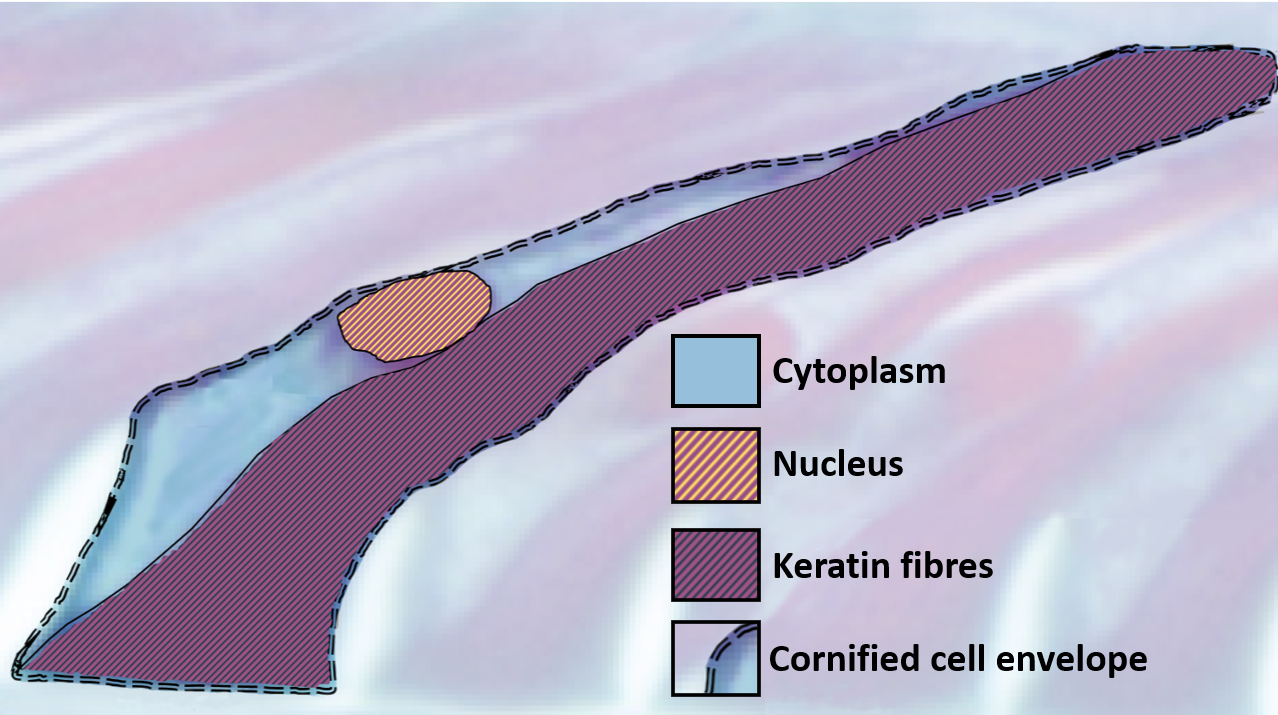
\includegraphics[width=0.60\linewidth, height=5.5cm, angle=0]{images/epidermal structure/cell_langowski_modified.PNG}
    \caption{Epithelial cell with the most important cell components.}
    \label{fig:epithelial_cell_components}
\end{figure}

 
\qquad The stiffness measurements on the tree frog can be compared to other stiffness measurements performed on animal tissue. The mechanical properties of animal tissue depend on the type of protein and on the level of hydration. One of the most frequent proteins is collagen. The fibers in the tree frog epithelial layer are composed of keratin which has a higher stiffness than collagen.\\
 
\qquad The stiffness for animal keratin in literature are given in Table \ref{tab:animal_keratin}. The animal keratin found in mammals can be classified as alpha or helical keratin while the keratin found in birds and reptiles can be classified as beta or pleated-sheet keratin \cite{bonser2000young}. The elastic properties of keratin in birds and reptiles are therefore considered more representative for the keratin properties of the tree frog. In the table below is also visible that the elastic moduli of the birds claw, the birds feathers and the gecko setae are very similar.\\

  
\begin{table}[h!]
\centering
\begin{tabular}{p{3cm}|p{2.5cm}|p{1cm}}
Origin                          & Elastic modulus [GPa]& Source                 \\
\hline
Sheep wool                      & 7-47              & \cite{simpson196551}\\
Human keratinocyte cytoskeleton & 1.2e-4 3.4e-4     & \cite{lulevich2010single}\\
Birds claw                      & 1.84              & \cite{bonser2000young}\\
Birds feathers                  & 2-5               & \cite{cameron2003young}\\
Gecko setae                     & 1.5               & \cite{peattie2007ancestrally}\\
Horse-hoof                      & 0.41 - 14.6       & \cite{bertram1987functional}
\end{tabular}
\caption{Stiffness values for animal and human keratin. The lower three rows give the stiffness values of pleated sheet keratin and are thus most relevant.}
\label{tab:animal_keratin}
\end{table}
  

\qquad The keratin fibers are embedded in connective tissue. Connective tissue typically has a lower stiffness than keratin but the exact composition of the connective tissue is not described in literature. Common connective tissue in bio-structures are collagen and elastin. The material properties of collagen are listed in Table \ref{tab:animal_collagen}. The collagen material properties are slightly lower but in the same range as the keratin material properties. This can be caused by the highly directional properties of the the tissues used to determine these stiffness values. Such directional properties are not visible in the material between the keratin fibers and above and below these fibers in the epithelial cell. The elastic properties of elastin indicate a much lower stiffness than the stiffness of collagen.\\ 

\begin{table}[h!]
\centering
\begin{tabular}{p{3cm}|p{2.5cm}|p{1cm}}
Origin                               & Elastic modulus [GPa] & Source                 \\
\hline
Collagen, rat tail tendon            & 3.75                  &\cite{wenger2007mechanical}\\
Collagen, bovine Achilles tendon     & 9.0                   &\cite{harley1977phonons}\\
Collagen, rat tail tendon            & 0.1 -0.36             &\cite{dutov2016measurement}\\  
Collagen, bovine Achilles tendon     & 0.002 - 0.2           &\cite{grant2009tuning}\\
Bovine elastin                       & 0.00041               &\cite{aaron1981elastin}\\
Bovine elastin                       & 0.0011                &\cite{gosline2002elastic}
\end{tabular}
\caption{Stiffness values for animal connective tissue.}
\label{tab:animal_collagen}
\end{table}


\qquad The stiffness values found in literature for collagen are relative close to the stiffness values found for keratin. The stiffness of these bio-materials however can be severely influenced by the degree of hydration. Grant et al. describes a range of $2-200 MPa$ for bovine collagen in varying solution conditions \cite{grant2009tuning} and Bertram et al. \cite{bertram1987functional} describes that the stiffness of horse-hoof keratin can be varied over a range of $0.41 - 14.6 GPa$  depending on the hydration of the material.\\ 

\qquad The relatively high stiffness measurements on hairs, claws, feathers and setae as visible in Table \ref{tab:animal_keratin} are all obtained from dead and relatively dry material. The stiffness of these materials is much higher than the stiffness of living keratinous material like keratinocytes as also visible in Table \ref{tab:animal_keratin}. These keratinocytes are much better hydrated than the dead keratinous materials. Furthermore, it should be noted that keratinocytes are living cells which also contain other cell elements which are most likely not as stiff as the keratinous elements in these cells. The stiffness of pure keratinous fibers is therefore expected to be in the range of $1-10 GPa$.\\ 

\qquad The exact composition of the connective tissue between the fibers is not reported in literature. Based on the stiffness values visible in Table \ref{tab:animal_collagen}, the stiffness of the connective tissue between the keratin fibers is most probable somewhere in between the stiffness values reported for collagen and elastin. Furthermore, the connective tissue in the epithelial cells is well hydrated. The effective stiffness of the connective tissue is therefore estimated at a range of $1-10 MPa$.\\

\qquad The most superficial layer of the cell epidermis outer epithelial layer of the adhesive pads is argued to have a relatively high stiffness \cite{nakano2016light}. This $10 nm$ thick layer is composed of insoluble proteins and its stiffness is most probable in the range of the keratinous cell elements.\\




% je kunt nog de literatuur in om strain stiffening voor keratine op te zoeken en daar dan ook weer een model van maken-is wel zo netjes



\section{Wet adhesive mechanism: theory and application}\label{sec:adhesive_theories}
% hier kunnen we dus ingaan op de bestaande theorien om de functie van de elementen in de poot van de kikker uit te leggen
% we doen de informatie die ik al opgezocht heb voor de literatuurstudie en vatten dit samen:
% -capillary forces en andere mechanisms die een rol spelen voor de 'natte' component
% - mechanismen die een rol spelen voor de droge adhesie
\subsection{Capillary forces}
The Laplace capillary force is defined as visible in Equation \ref{eq:laplace_capillary_general} \cite{laplace1799traite}. With $\gamma$ for the surface tension, $\Delta P$ for the pressure difference and $R_1$ and $R_2$ for the radii of the two contact surfaces that are involved in the contact. When these radii become very large, the liquid volume needed between the two surfaces is reduced to almost zero, increasing the value of the capillary pressure difference $\Delta P$. The minimum amount of adhesive liquid between two surfaces is dependent on the degree of roughness of these surfaces \cite{qian2006scaling}. The limit of the pad-substrate gap size reduction is at the critical length for which the fluid itself would fail due to cavitation. Very thin fluid layers can also lead to unstable spreading and shrinking of the fluid layer \cite{yi2009dynamic} and are thus undesirable for the generation of stable adhesive forces.\\ 
\begin{equation}
    \Delta P = - \gamma (\frac{1}{R_1} + \frac{1}{R_2})
    \label{eq:laplace_capillary_general}
\end{equation}

\qquad The Another factor of influence in capillary adhesion is the contact angle. An increase in the contact angle generally results in an increase in the required liquid volume to establish full contact and with that reduce adhesion \cite{qian2006scaling}. It is found that an adhesive pad will always achieve the maximum adhesive strength and robustness when the effective contact angle is smaller than a critical value \cite{su2009concave}. For flat contact surfaces, this critical angle is around 30 degrees \cite{orchard2012influence}. Su et al. discovered that a concave pad geometry transfers the contact angle to a smaller contact angle. This concave geometry increases the critical contact angle to a value of 45 degrees.\\

\qquad The role of the surface tension is still under discussion. According to Smith et al.  \cite{smith2006adhesion} the magnitude of the capillary forces can be explained by a presence of a surface tension based force \cite{peng2016microstructure}.  This capillary force depends on the amount of liquid bridges formed, the volume of the individual droplets and on the contact angles from the droplets to the substrate and to the adhesive pad. Others however state that the tenacities measured for tree frogs are in the same range as capillary forces measured between two glass plates \cite{langowski2018tree}. This suggests that there is only one continuous liquid meniscus between the two surfaces \cite{scholz2009ultrastructure} which makes that the surface tension contribution can not be considered as significant since it is dependent on the amount of liquid bridges formed.\\

\qquad The secretion fluids are an emulsion of hydrophilic and hydrophobic components. This emulsion is able to stick well to hydrophilic and hydrophobic surfaces \cite{langowski2018tree}. The hydrophobic or hydrophilic pad properties can have a severe influence on the adhesive performance for large contact angles. For contact angles below the critical value of 30 degrees the hydrophobic or hydrophilic surface properties do not severely change the adhesive pad properties \cite{orchard2012influence}.\\

\subsection{Van der Waals forces}
\qquad Although capillary forces are considered the main adhesional mechanism for tree frogs, there are also measurements that indicate the existence of dry contact interaction between adhesional pads and substrate \cite{kappl2016nanoscale}. These dry contacts do most likely occur on epithelial cell borders and at the location of nanopillars that come close enough to the substrate to establish dry contact. Dry contact allows Van der Waals forces to play a role. These contact forces can also play a role in very thin liquid layers though molecular ordering and interaction in the fluid \cite{federle2004biomechanics}. Dry contact interaction through Van der Waals forces is furthermore dependent on the temperature, ambient humidity and on the sliding velocity for sliding contacts.\\ 

\qquad The forces involved in dry contact interaction can be calculated with the Kendall equation which represents a peeling model for sticky rubber tape as visible in Equation \ref{eq:Kendall_equation}. This equation calculates the work of adhesion $W_a$ with the applied force $F$, the peeling angle $\alpha$, $d$ for the width of the tape with a Young's modulus $E$. According to this equation, friction forces are high for small values for $\alpha$. The force scales with the width of the tape because the peeling stress concentrations are found on the edges of the tape under peeling stress. This contact angle dependence is also observed in the previous section about capillary adhesion. A low contact angle can also cause crack healing to occur for critical peeling force values.\\
\begin{equation}
    W_a = F(1-cos(\alpha)) + \frac{F^2}{2dE}
    \label{eq:Kendall_equation}
\end{equation}

\subsection{Tree frog inspired applications}\label{sec:tree_frog_applications}
\qquad The work by Xue et al. describes an application of an fiber re-enforced material inspired on the toe pads of tree frogs. This work describes the difference in stress the distribution in the composite material between a fiber re-enforced material in which the fibers and the base material are properly attached to each other and a material in which the fibers and the base material are not bound to each other. The adhesional performance of both materials is evaluated with a measurement of the vertical pull-of force needed to release the material from a substrate. The materials where compressed into the substrate prior to the pull-of force measurement.\\

\qquad The results obtained by Xue show that the stress in the composite in which the base material and the fibers are properly bound has a much lower maximum value. Furthermore, the maximum stress is not located at the edge of the geometry but can be found at a certain distance(1-2 rows of pillars from the edge) from the material edge. A composite material in which the fibers are not bound to the base material has a maximum stress on the edge of the geometry as is also the case for homogeneous materials. The stress distributions for the material with the well-bound and the loose fibers are visible in Figure \ref{fig:Xue_model_1} and \ref{fig:Xue_model_2} respectively.\\ 

\begin{figure}[h!] 
    \begin{subfigure}{0.49\textwidth}
    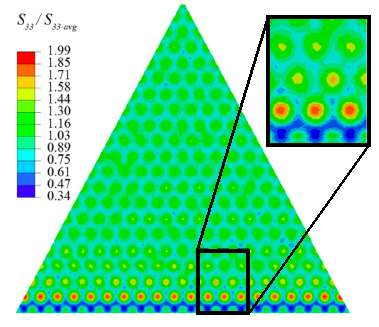
\includegraphics[width=\linewidth, height=6cm, angle=0]{images/Xue_work/Xue_model_internal_bounding.png}
    \caption{}
    \label{fig:Xue_model_1}
    \end{subfigure}
        \hfill
    \begin{subfigure}{0.49\textwidth}
    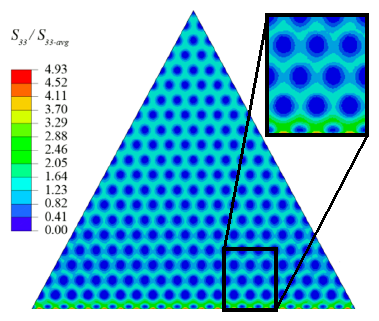
\includegraphics[width=\linewidth, height=6cm, angle=0]{images/Xue_work/Xue_model_internal_loose.png}
    \caption{}
    \label{fig:Xue_model_2}
    \end{subfigure}
    \caption{Pictures from the modeling work by Xue et al. The stress distribution in (a) is the result of the internal bounding between the fibers and the base material. The stress distribution in (b) has a larger stress peak on the edge of the geometry. This is due to the absence of internal bounding between the fibers and the base material. It should be noted that only the $S_{33}$ component is taken into account.}
    \label{fig:all_images_Xue}
\end{figure}

\qquad The explanation for the difference in stress distribution between the two materials is that the well-bound fibers are better able to distribute the stress over the material domain. The stress concentrations in Figure \ref{fig:Xue_model_1} are located at the top of the nanopillars. This is caused by the transfer of stress from the contact surface to the relatively stiff fibers which bear more stress than the base material. The stress concentrations we see on the edges of the domain for the material with the loose fibers in Figure \ref{fig:Xue_model_2}, are transferred to the fibers for the material in which the fibers are well-bound to the relatively soft material surrounding the fibers. This reduces the magnitude of the stress concentrations and slows down the development of cracks between the material and the substrate that would ultimately lead to detachment from the substrate. Furthermore do friction experiments show increased frictional performance for materials with well-bound fibers when compared to materials without or loose fibers.






\section{Goal of the research}\label{sec:goal}
\section{Report outline}\label{sec:outline}